%%%-------------------------------------------------------------------------
%%% PD3予稿集テンプレート (main.tex)
%%% 作成: 金沢工大・情報工学科・鷹合研究室(2017,12/6)
%%%-------------------------------------------------------------------------

%%%%%%%%%%%%%%%%%%%%%%%%%%%%%%%%%%%%%%%%%%%%%%%%%%%%%%%%%%%%%%%%%%%%%%%%%%%
%                               テーマ,著者情報をここに書き込んでください
%ここから ------------------------------------------------------------------

%%% テーマ番号
\def\THEMEID{XYZ-1234}

%%% 「テーマ番号」の配置を右寄せにするときはコメントにしてください
\def\RHEADER{}

%%% タイトル
\def\TITLEJP{誤差伝播モデルに基づく最適な整数対整数変換の構成法}
\def\TITLEEN{A Construction Method of Optimum Integer-to-integer Transform based on an Error Propagation Model}
\def\CENTERADJ{4} % 和文と英文で使われた行数をここに書き込んで下さい.

%%% 教員名
\def\PROFNAME{福沢 諭吉 教授}

%%% アブストラクト
\def\ABSTRACT{
ここにアブストラクトを書いてください(5行くらいか).あいうえおかきくけこさしすせそたちつてとなにぬねのはひふへほまみむめもやゆよらりるれろわをん.あいうえおかきくけこさしすせそたちつてとなにぬねのはひふへほまみむめもやゆよらりるれろわをん.あいうえおかきくけこさしすせそたちつてとなにぬねのはひふへほまみむめもやゆよらりるれろわをん.あいうえおかきくけこさしすせそたちつてとなにぬねのはひふへほまみむめもやゆよらりるれろわをん.
}

%%% キーワード
\def\KEYWORDS{qwerty,qwerty,qwerty,qwerty,qwerty,qwerty,qwerty}

%%% 著者リスト
\def\AUTHORS{
\begin{tabular}{llcll}
 4EP5-4  & 織田 信長(Nobunaga Oda)      && 4EP5-11  & 松永 久秀(Hisahide Matsunaga)\\
 4EP5-29 & 筒井 順慶(Junkei Tsutsui)    && 4EP5-100 & 百地 丹波(Tanba Momochi)\\
\end{tabular}}

% テーマ,著者情報ここまで -----------------------------------------------------


%%%%%%%%%%%%%%%%%%%%%%%%%%%%%%%%%%%%%%%%%%%%%%%%%%%%%%%%%%%%%%%%%%%%%%%%%%%%
%                                本文
\documentclass{tkglabs} 
\begin{document}       
\maketitle
\begin{multicols*}{2} % *アスタ付きだとページのバランシングを無効にできる 
%本文ここから ------------------------------------------------------------------




\section{はじめに}
背景や目的をここに書いてください.あいうえおかきくけこさしすせそたちつてとなにぬねのはひふへほまみむめもやゆよらりるれろわをん.あいうえおかきくけこさしすせそたちつてとなにぬねのはひふへほまみむめもやゆよらりるれろわをん.

\section{全天球カメラ画像の球面マッピング法}
早春の暖かい光が地上の全ての生き物に降り注いでいます(徳田小学校卒業式送辞).早春の暖かい光が地上の全ての生き物に降り注いでいます(徳田小学校卒業式送辞)早春の暖かい光が地上の全ての生き物に降り注いでいます(徳田小学校卒業式送辞)早春の暖かい光が地上の全ての生き物に降り注いでいます(徳田小学校卒業式送辞)
\subsection{従来法}
早春の暖かい光が地上の全ての生き物に降り注いでいます(徳田小学校卒業式送辞).早春の暖かい光が地上の全ての生き物に降り注いでいます(徳田小学校卒業式送辞)早春の暖かい光が地上の全ての生き物に降り注いでいます(徳田小学校卒業式送辞)早春の暖かい光が地上の全ての生き物に降り注いでいます(徳田小学校卒業式送辞)
\subsection{提案法}
早春の暖かい光が地上の全ての生き物に降り注いでいます(徳田小学校卒業式送辞).早春の暖かい光が地上の全ての生き物に降り注いでいます(徳田小学校卒業式送辞)早春の暖かい光が地上の全ての生き物に降り注いでいます(徳田小学校卒業式送辞)早春の暖かい光が地上の全ての生き物に降り注いでいます(徳田小学校卒業式送辞)早春の暖かい光が地上の全ての生き物に降り注いでいます(徳田小学校卒業式送辞).早春の暖かい光が地上の全ての生き物に降り注いでいます(徳田小学校卒業式送辞)早春の暖かい光が地上の全ての生き物に降り注いでいます(徳田小学校卒業式送辞)早春の暖かい光が地上の全ての生き物に降り注いでいます(徳田小学校卒業式送辞)早春の暖かい光が地上の全ての生き物に降り注いでいます(徳田小学校卒業式送辞).早春の暖かい光が地上の全ての生き物に降り注いでいます(徳田小学校卒業式送辞)早春の暖かい光が地上の全ての生き物に降り注いでいます(徳田小学校卒業式送辞)早春の暖かい光が地上の全ての生き物に降り注いでいます(徳田小学校卒業式送辞)
\section{文章の書き方}
\subsection{図表の書き方,相互参照}
核融合の仕組みをFig.\ref{FIG_KUJIRA}に示す\cite{jp2k1,jp2k2}.核融合の仕組みをFig.\ref{FIG_CAT}に示す.Table\ref{TBL_XYZ}は今年食べて美味しかった果物を示したものである\cite{sdkguide}.
\begin{Figure}
	\centering
	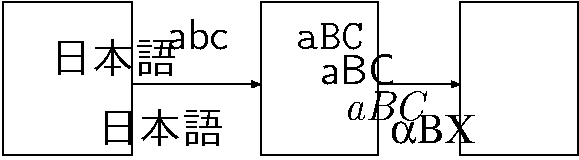
\includegraphics[width=\linewidth]{fig/concept.pdf}
	\captionof{figure}{ダイオウイカとマッコウクジラ}\label{FIG_KUJIRA}
\end{Figure}


\begin{Figure}
	\centering
	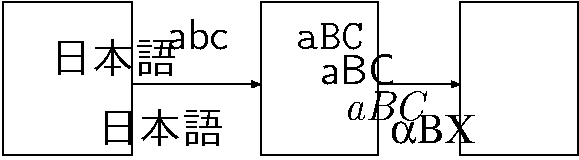
\includegraphics[width=\linewidth]{fig/concept.pdf}
	\captionof{figure}{ベルクカッツェと山猫の関係}\label{FIG_CAT}
\end{Figure}


\begin{Table}
	\centering
	\captionof{table}{裏帳簿}\label{TBL_XYZ}
	\vspace{-2mm}
	\begin{tabular}{|l|l|l|}
		\hline
			なまえ & 味 & 産地\\
		\hline
				リンゴ & 92.1 & 青森\\
				みかん & 92.6 & 愛媛\\
				いちご & 90.3 & 金沢\\
		\hline
	\end{tabular}
\end{Table}
\subsection{箇条書き}
あああああああああああああ
\subsubsection{番号付き箇条書き}
番号付きの場合は以下のようにする.番号付きの場合は以下のようにする.番号付きの場合は以下のようにする.
\begin{enumerate}
 \item あああああああ
\item いいいいいいい
\item うううううう
\item ええええええ
\end{enumerate}
ああああああああああああああああああああああああああああああああああああああああああああああああああああああああああああああああああああああ
\subsubsection{見出し付き箇条書き}
見出し付きの場合は以下のようにする.
\begin{description}
 \item[あああああああ]おおおおおおおおおおおお
 \item[いいいいいいい]いいいいいいいいいいいいい
 \item[うううううう]うううううううううううううううううううううううううううううううううううううううううううううううううううううううううううう
 \item[ええええええ]ああああああああああああああああああああああああああああああああああああああああああああああああああああああああ
\end{description}
\section{システム構成}
	あいうえおかきくけこさしすせそたちつてとなにぬねのはひふへほまみむめもやゆよらりるれろわをん.あいうえおかきくけこさしすせそたちつてとなにぬねのはひふへほまみむめもやゆよらりるれろわをん.あいうえおかきくけこさしすせそたちつてとなにぬねのはひふへほまみむめもやゆよらりるれろわをん.あいうえおかきくけこさしすせそたちつてとなにぬねのはひふへほまみむめもやゆよらりるれろわをん.ああああああああああああああああああああああああああああああああああああああああああああああああああああああああああああああああああああ.あいうえおかきくけこさしすせそたちつてとなにぬねのはひふへほまみむめもやゆよらりるれろわをん.あいうえおかきくけこさしすせそたちつてとなにぬねのはひふへほまみむめもやゆよらりるれろわをん.あいうえおかきくけこさしすせそたちつてとなにぬねのはひふへほまみむめもやゆよらりるれろわをん.あいうえおかきくけこさしすせそたちつてとなにぬねのはひふへほまみむめもやゆよらりるれろわをん.
	\section{評価実験の方法}
	あいうえおかきくけこさしすせそたちつてとなにぬねのはひふへほまみむめもやゆよらりるれろわをん.あいうえおかきくけこさしすせそたちつてとなにぬねのはひふへほまみむめもやゆよらりるれろわをん.あいうえおかきくけこさしすせそたちつてとなにぬねのはひふへほまみむめもやゆよらりるれろわをん.あいうえおかきくけこさしすせそたちつてとなにぬねのはひふへほまみむめもやゆよらりるれろわをん.ああああああああああああああああああああああああああああああああああああああああああああああああああああああああああああああああああああ.あいうえおかきくけこさしすせそたちつてとなにぬねのはひふへほまみむめもやゆよらりるれろわをん.あいうえおかきくけこさしすせそたちつてとなにぬねのはひふへほまみむめもやゆよらりるれろわをん.あいうえおかきくけこさしすせそたちつてとなにぬねのはひふへほまみむめもやゆよらりるれろわをん.あいうえおかきくけこさしすせそたちつてとなにぬねのはひふへほまみむめもやゆよらりるれろわをん.	あいうえおかきくけこさしすせそたちつてとな
	
		\section{実験結果}
	あいうえおかきくけこさしすせそたちつてとなにぬねのはひふへほまみむめもやゆよらりるれろわをん.あいうえおかきくけこさしすせそたちつてとなにぬねのはひふへほまみむめもやゆよらりるれろわをん.あいうえおかきくけこさしすせそたちつてとなにぬねのはひふへほまみむめもやゆよらりるれろわをん.あいうえおかきくけこさしすせそたちつてとなにぬねのはひふへほまみむめもやゆよらりるれろわをん.ああああああああああああああああああああああああああああああああああああああああああああああああああああああああああああああああああああ.あいうえおかきくけこさしすせそたちつてとなにぬねのはひふへほまみむめもやゆよらりるれろわをん.あいうえおかきくけこさしすせそたちつてとなにぬねのはひふへほまみむめもやゆよらりるれろわをん.あいうえおかきくけこさしすせそたちつてとなにぬねのはひふへほまみむめもやゆよらりるれろわをん.	
	\section{考察}
		あいうえおかきくけこさしすせそたちつてとなにぬねのはひふへほまみむめもやゆよらりるれろわをん.あいうえおかきくけこさしすせそたちつてとなにぬねのはひふへほまみむめもやゆよらりるれろわをん.あいうえおかきくけこさしすせそたちつてとなにぬねのはひふへほまみむめもやゆよらりるれろわをん.あいうえおかきくけこさしすせそたちつてとなにぬねのはひふへほまみむめもやゆよらりるれろわをん.ああああああああああああああああああああああああああああああああああああああああああああああああああああああああああああああああああああ.あいうえおかきくけこさしすせそたちつてとなにぬねのはひふへほまみむめもやゆよらりるれろわをん.あいうえおかきくけこさしすせそたちつてとなにぬねのはひふへほまみむめもやゆよらりるれろわをん.あいうえおかきくけこさしすせそたちつてとなにぬねのはひふへほまみむめもやゆよらりるれろわをん.あいうえおかきくけこさしすせそたちつてとなにぬねのはひふへほまみむめもやゆよらりるれろわをん.
	\section{まとめ}
		あいうえおかきくけこさしすせそたちつてとなにぬねのはひふへほまみむめもやゆよらりるれろわをん.あいうえおかきくけこさしすせそたちつてとなにぬねのはひふへほまみむめもやゆよらりるれろわをん.あいうえおかきくけこさしすせそたちつてとなにぬねのはひふへほまみむめもやゆよらりるれろわをん.あいうえおかきくけこさしすせそたちつてとなにぬねのはひふへほまみむめもやゆよらりるれろわをん.


%% 参考文献(必要に応じて追加)
\begin{thebibliography}{99}
\bibitem{jp2k1} 織田 信長, 明智 光秀, "JPEG2000画像符号化システムにおける係数ビットモデリングと適応算術符号化,"Journal of signal processing(基礎シリーズ), vol.7, no.4, pp.257-266, July 2003.
\bibitem{jp2k2} 織田 信長, 明智 光秀, "JPEG2000画像符号化システムにおける係数ビットモデリングと適応算術符号化 -II,"Journal of signal processing(基礎シリーズ), vol.7, no.5, pp.337-349, Sept. 2003.
\bibitem{sdkguide}Parrot, "AR.Drone Developer Guide SDK 2.0"
\bibitem{bk1} "金沢の暮らし", \url{http://www.kanazawa-it.ac.jp}
\bibitem{bk2} 山田 太郎, "金沢の一人暮らし", トンチンカン出版, 2016.
\end{thebibliography}


% 本文ここまで ------------------------------------------------------------------
\end{multicols*} 
\end{document}

